\documentclass{article}
\usepackage[OT1]{fontenc}
\usepackage{graphicx}
\usepackage{setspace}
\usepackage{anysize}
\usepackage{enumerate}
\usepackage{amssymb}
\usepackage{algorithm2e}
\usepackage{amsthm}
\usepackage{amsmath}
\usepackage{booktabs}
\usepackage{ulem}
\marginsize{3cm}{3cm}{0cm}{3cm}

\fontfamily{ptm}\fontsize{14}{14}\selectfont 
\singlespacing
\newcommand{\solution}[1]{~\\ $\blacksquare$ \sffamily\upshape\selectfont #1
\normalfont ~\\~ }
\newcommand\independent{\protect\mathpalette{\protect\independenT}{\perp}}
\def\independenT#1#2{\mathrel{\rlap{$#1#2$}\mkern2mu{#1#2}}} 
\setlength{\parindent}{0pt}
% \setlength{\textwidth}{1.5\textwidth}

\begin{document}
\begin{center}
\textbf{\large{
HOMEWORK 3 \\
Introduction to Artifitial Intelligence \\}}
\textsc{\Large{Shumin Guo}}
\end{center}

\section{Execise 20.9}
Consider a single Boolean random variable $Y$ (the
"classification"). Let the prior probability P(Y = $true$) be $\pi$. Let's 
try to find $\pi$, given a training set $D=(y_1,\ldots,y_N)$ with N
independent samples of Y. Furthermore, suppose $p$ of the $N$ are positive
and $n$ of the $N$ are negative.
\begin{enumerate}[a.]
\item Write down an expression for the likelihood of D (i.e., the
probability of seeing this particular sequence of examples, given a
fixed value of $\pi$) in terms of $\pi$, and $n$.
\solution{
  $L(\pi) = \pi^n(1-\pi)^{N-n}$
}
\item By differentiating the log likelihood L, find the value of $\pi$
that maximizes the likelihood.
\solution{
  \begin{align*}
    \pi^{mle}&=\arg\max_{\pi}\pi^p(1-\pi)^n \\
    &= \arg\max_{\pi}plog\pi+nlog(1-\pi) \\
    &= \pi ~s.t.~ \frac{\partial LL}{\partial \pi} = 0 \\ 
    &= \pi ~s.t.~ p\frac{1}{\pi}+n\frac{1}{1-\pi} = 0 \\
    &= \frac{p}{n+p}
  \end{align*}
}
\item Now suppose we add in $k$ Boolean random variables $X_1, X_2,\ldots,X_k
$ (the "attributes") that describe each sample. and suppose we assume
that the attributes are conditionally independent of each other given
the goal Y. Draw the Bayes net corresponding to this assumption.
\solution{
See Bayesian network in Figure \ref{fig:20_1c}.
  \begin{figure}[ht]
    \centering
    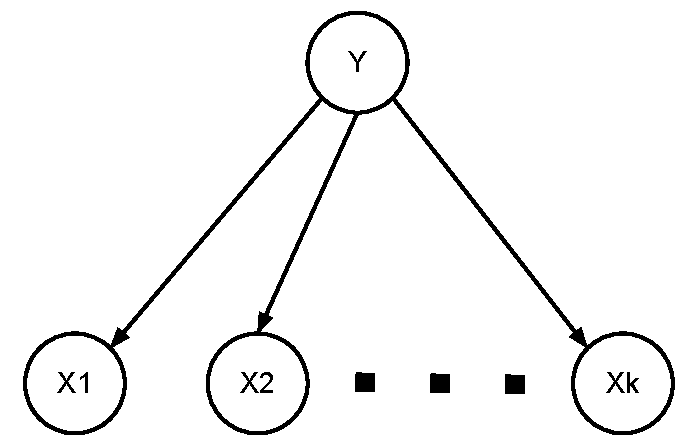
\includegraphics[width=.5\textwidth]{AI-HWK3_1c.pdf}
    \caption{Bayesian Network for question c.}\label{fig:20_1c}
  \end{figure}
}
\item Write down the likelihood for the data including the attributes,
using the following additional notation:
\begin{itemize}
\item $\alpha_i$ is $P(X_i=true|Y=true)$.
\item $\beta_i$ is $P(X_i = true|Y = false)$.
\item $p_i^+$ is the count of samples for which $X_i = true$ and $Y = true$.
\item $n_i^+$ is the count of samples for which $X_i = false$ and $Y = true$.
\item $p_i^-$ is the count of samples for which $X_i = true$ and $Y = false$.
\item $n_i^-$ is the count of samples for which $X_i = false$ and $Y = false$.
\end{itemize}

[Hint: consider first the probability of seeing a single example with
specified values for $X_1, X_2,\ldots,X_k$ and $Y$.]
\solution{
  We use Y to denote $Y=true$ $\neg Y$ to denote $Y=false$, $X_i$ to denote
  $X_i=true$ and $\neg X_i$ to denote $X_i=false$. 
  \begin{align*}
    & P(x_{11},\ldots,x_{1k},\ldots,x_{N1},\ldots,x_{Nk},y_1,\ldots,y_N) \\
    & = \prod_{i=1}^N\prod_{j=1}^kP(x_{ij}|y_i)P(y_i) \\
    & = (\prod_{i=1}^NP(y_i))(\prod_{j=1}^k(\prod_{i=1}^pP(x_{ij}|y_i))(\prod_{i=1}^nP(x_{ij}|y_i))) \\
    & = \pi^p(1-\pi)^n(\prod_{j=1}^k(\prod_{i=1}^{p_j^+}P(x_{ij}|y_i))(\prod_{i=1}^{n_j^+}P(x_{ij}|y_i)) 
    (\prod_{i=1}^{p_j^-}P(x_{ij}|y_i))(\prod_{i=1}^{n_j^-}P(x_{ij}|y_i)) \\
    & = \pi^p(1-\pi)^n(\prod_{j=1}^k(\prod_{i=1}^{p_j^+}P(X_j|Y))(\prod_{i=1}^{n_j^+}P(\neg X_j|Y)) 
    (\prod_{i=1}^{p_j^-}P(X_j|\neg Y))(\prod_{i=1}^{n_j^-}P(\neg X_j|\neg Y)) \\
    & = \pi^p(1-\pi)^n\prod_{j=1}^k\alpha_j^{p_j^+}(1-\alpha_j)^{n_j^+}\beta_j^{p_j^-}(1-\beta_j)^{n_j^-} \\
    &\mbox{\rmfamily\selectfont{By replacing j to i.}\normalfont} \\
    & = \pi^p(1-\pi)^n\prod_{i=1}^k\alpha_i^{p_i^+}(1-\alpha_i)^{n_i^+}\beta_i^{p_i^-}(1-\beta_i)^{n_i^-} 
  \end{align*}
}

\item By differentiating the log likelihood L, find the values of
  $\alpha_i$ and $\beta_i$ (in terms of the various counts) that
  maximize the likelihood and say in words what these values represent.
\solution{
  \begin{align*}
    LL & = plog\pi + nlog(1-\pi) + \sum_{i=1}^k(p_i^+log\alpha_i + n_i^+log(1-\alpha_i) 
    + p_i^-log\beta_i + n_i^-log(1 - \beta_i)) \\ 
    \frac{\partial(LL)}{\partial\alpha_i} & = \sum_{i=1}^k(\frac{p_i^+}{\alpha_i} 
    - \frac{n_i^+}{1-\alpha_i}) = 0  \\
    &\Rightarrow \alpha_i=\frac{p_i^+}{p_i^++n_i^+} \\
    \frac{\partial(LL)}{\partial\beta_i} &= \sum_{i=1}^k(\frac{p_i^-}{\beta_i} 
    - \frac{n_i^-}{1-\beta_i}) = 0  \\
    &\Rightarrow \beta_i = \frac{p_i^-}{p_i^-+n_i^-}
  \end{align*}
  Explanations: $\alpha_i$ is the ratio of $X_i=true$ when $Y=true$ and Similarly, 
  $\beta_i$ is the ratio of $X_i=true$ when $Y=false$. 
}
\item Let $k = 2$, and consider a data set with 4 all four possible
examples of the \textsc{Xor} function. Compute the maximum likelihood
estimates of $\pi, \alpha_1, \alpha_2, \beta_1$ and $\beta_2$.
\solution{
  Samples can be found in Table \ref{tbl:1-f}. 
  \begin{table}[h]
    \centering
    \begin{tabular}{ccc}
      \toprule
      \textbf{$X_1$} & \textbf{$X_2$} & \textbf{$Y$} \\ \toprule
      0 & 0 & 0 \\ \midrule
      0 & 1 & 1 \\ \midrule
      1 & 0 & 1 \\ \midrule
      1 & 1 & 0 \\ \bottomrule
    \end{tabular}
    \caption{Sample data using XOR function.}
    \label{tbl:1-f}
  \end{table}

  According to the sample data, we can get the counts as follows: 
  \[p_1^+=1, p_2^+=1, n_1^+=1, n_2^+=1, p_1^-=1, p_2^-=1, n_1^-=1, n_2^-=1\].
  And the maximum likelihood values are: \[\pi = 0.5, \alpha_1 = 0.5, 
  \alpha_2 = 0.5, \beta_1 = 0.5, \beta_2 = 0.5.\]
}
\item Given these estimates of $\pi, \alpha_1, \alpha_2, \beta_1$ and
  $\beta_2$, what are the posterior probabilities $P(Y = true|x_1,x_2)$
  for each example? 
\solution{
  \begin{align*}
    P(Y|x_1,x_2) & = \frac{P(x_1,x_2|Y)P(Y)}{P(x_1,x_2)} \\ 
    & = \frac{P(x_1|Y)P(x_2|Y)P(Y)}{P(x_1)P(x_2)} ~ where ~ P(x_1=1) = P(x_2=1) = 0.5\\ 
    & = \frac{0.5\times 0.5\times 0.5}{0.5\times 0.5} \\ 
    & = 0.5 
  \end{align*}
  The posterior probability $P(Y=true|x_1,x_2) = 0.5$ for all the examples.
}
\end{enumerate}

\section{Execise 2.}
\[ p(x|\mu_1,\mu_2)=\frac{1}{3}\sqrt{2\pi}exp(-\frac{1}{2}(x-\mu_1)^2) +
\frac{2}{3\sqrt{2\pi}}exp(-\frac{1}{2}(x-\mu_2)^2) \]
The 25 samples (0.608,-1.590, 0.235, 3.949,-2.249, 2.704,-2.473,
0.672, 0.262, 1.072,-1.773, 0.537, 3.240, 2.400,-2.499, 2.608,-3.458,
0.257, 2.569, 1.415, 1.410,-2.653, 1.396, 3.286,-0.712) were drawn
from this mixture with mean $\mu_1$ = -2 and $\mu_2$ = 2. Using these
25 samples to estimate $\mu_1$ and $\mu_2$ by maximum likelihood
principle through EM algorithm with initial values (a)
$\hat{\mu}^{(0)} = 1$ and $\hat{\mu}^{(2)=3}$; $(b)\hat{\mu}^{(0)} =
4$ and $\hat{\mu}^{(2)} = -3$; (c) $\hat{\mu}^{(0)} = -2$ and
$\hat{\mu}^{(2)} = -2$; (d) $\hat{\mu}^{(0)} = 5$ and $\hat{\mu}^{(2)}
= 5$. Are they the same? Please explain.
\solution{

}
\section{Execise 15.13}
A professor wants to know if students are getting enough sleep. Each
day, the professor observes whether the students sleep in class, and
whether they have red eyes. The professor has the following domain
theory:
\begin{itemize}
\item The prior probability of getting enough sleep, with no
  observations, is 0.7.
\item The probability of getting enough sleep an night $t$ is 0.8 given
  that the student got enough sleep the previous night, and 0.3 if not. 
\item The probability of having red eyes is 0.2 if the student got
  enough sleep, and 0.7 if not. 
\item The probability of sleeping in class is 0.1 if the student got
  enough sleep, and 0.3 if not. 
\end{itemize}
Formulate this information as a dynamic Bayesian network that the
professor could use to filter or predict from a sequence of
observations. Then reformulate it as a hidden Markov model that has
only a single observation variable. Give the complete probability
tables for the model.

\section{Execise 15.14}
For the DBN specified in Exercise 15.13 and for the evidence values \\
$e_1 =$ not red eyes, not sleeping in class \\
$e_2 =$ red eyes, not sleeping in class \\
$e_3 =$ red eyes, sleeping in class \\
perform the following computations:
\begin{enumerate}[a.]
\item State estimation: Compute $P(EnoughSleep_t|e_{1:t})$ for each
  of $t = 1, 2, 3$.
\item Smoothing: Compute $P(EnoughSleep_t|e_{1:3})$ for each of $t = 1,2,3$.
\item Compare the filtered and smoothed probabilities for $t = 1$ and $t = 2$.
\end{enumerate}

\section{Execise 15.15}
Suppose that a particular student shows up with red eyes and sleeps in
class every day. Given the model described in Exercise 15.13, explain
why the probability that the student had enough sleep the previous
night converges to a fixed point rather than continuing to go down as
we gather more days of evidence. What is the fixed point? Answer this
both numerically (by computation) and analytically.

\end{document}